\section{Trabalhos Relacionados \label{sec:trab_rel}}

\subsection*{Introdução}

\subsubsection*{Descrição geral do que tratará esta seção}
\subsubsection*{Organização desta seção}

\subsection{Aplicativos, websites e sistemas em geral \label{subsec:app_web}}

Com o aumento do poder computacional devido ao advento das Unidades de Processamento Gráfico (GPUs), o uso de Redes Neurais para identificar objetos em imagens tornou-se viável. 
Empresas como Google, Amazon e Microsoft, juntaram suas pesquisas em reconhecimento de imagem em APIs (Application Programming Interfaces) para que os desenvolvedores de software possam usar essa tecnologia em aplicativos. As APIs são as seguintes: Google Vision API, Amazon Rekognition, e Microsoft Computer Vision API.

A Google Vision API \cite{google_vision} oferece funções de visão computacional para as imagens que você envia para a API e permite que os desenvolvedores integrem facilmente recursos de detecção de visão em aplicativos, incluindo rotulação de imagens, detecção de face e ponto de referência, reconhecimento ótico de caracteres (OCR) e marcação de conteúdo explícito, isto é a API também pode detectar conteúdo inadequado em imagens usando os mesmos modelos de aprendizado de máquina que potencializam o Google SafeSearch. 
%https://cloud.google.com/blog/products/gcp/filtering-inappropriate-content-with-the-cloud-vision-api

O Amazon Rekognition \cite{amazon_rekognition} é um sofisticado serviço deep learning da Amazon Web Services (AWS) que facilita a adição de análises de imagens e vídeos a aplicativos. Basta fornecer uma imagem ou vídeo à API do Rekognition e o serviço poderá identificar objetos, cenas, rostos, celebridades e conteúdo inadequado dentro das imagens. Além disso, o Amazon Rekognition oferece análise e reconhecimento facial altamente precisos para suas imagens e vídeos. Você pode detectar, analisar e comparar faces para uma grande variedade de casos de uso de verificação de usuários, contagem de pessoas e segurança pública.

O Microsoft Computer Vision API \cite{azure_microsoft_computer_vision} pertence a um conjunto de ferramentas da Microsoft, chamado de Microsoft Cognitive Services. O Microsoft Cognitive Services são APIs, SDKs e serviços disponíveis para ajudar os desenvolvedores a criarem aplicativos inteligentes pois permite aos desenvolvedores adicionar facilmente aos seus aplicativos recursos cognitivos como emoção e detecção de vídeo, reconhecimento facial, de fala e de visão, além de compreensão de fala e de idioma. O objetivo é oferecer diversos serviços cognitivos para diferentes áreas como visão, fala, pesquisa, conhecimento e idiomas. O Computer Vision API pertence à área de visão e fornece aos desenvolvedores o acesso a algoritmos avançados para processar imagens e retornar informações. Ao carregar uma imagem ou especificar uma URL de imagem, algoritmos podem analisar o conteúdo visual de maneiras diferentes com base em entradas e nas opções do usuário.

Aplicativos de perda de peso, em que há um acompanhamento das refeições feitas durante o dia, existem há anos, mas exigiam que os usuários inserissem manualmente o que estavam comendo em seus bancos de dados para rastrear as calorias e os valores nutricionais dos alimentos. Hoje em dia, existem softwares que já fazem o reconhecimento de imagens e são capazes de identificar o alimentos presentes em uma foto.

O Calorie Mama \cite{caloriemama_2016} é um aplicativo para celular que promete exatamente isso. Basta tirar uma foto da comida para obter as informações nutricionais da refeição. O Calorie Mama utiliza o Food AI API para reconhecimento dos itens alimentares nas imagens.

O aplicativo Lose It \cite{lose_it} também promete a mais avançada tecnologia de reconhecimento de imagem para oferecer a melhor experiência de rastreamento de alimentos no mundo através de um recurso chamado Snap It.

A figura \ref{fig:apps} mostra o funcionamento dos dois aplicativos. A figura \ref{fig:subApps1} mostra a tela do Calorie Mama, onde a figura utilizada foi de um prato de macarrão. Percebe-se que a sugestão dada pelo aplicativo é a categoria "pasta" que significa "massa" em português. O mesmo acontece para a figura \ref{fig:subApps2}, em que é utilizada a mesma imagem, mas no Lose It e a categoria que foi sugerida pelo aplicativo é também "pasta".

\begin{figure}[!ht] 
\centering
\caption{Comparação entre os aplicativos.}
\label{fig:apps}
\begin{subfigure}{0.4\textwidth}
  \centering
    \caption{Aplicativo Calorie Mama.}
   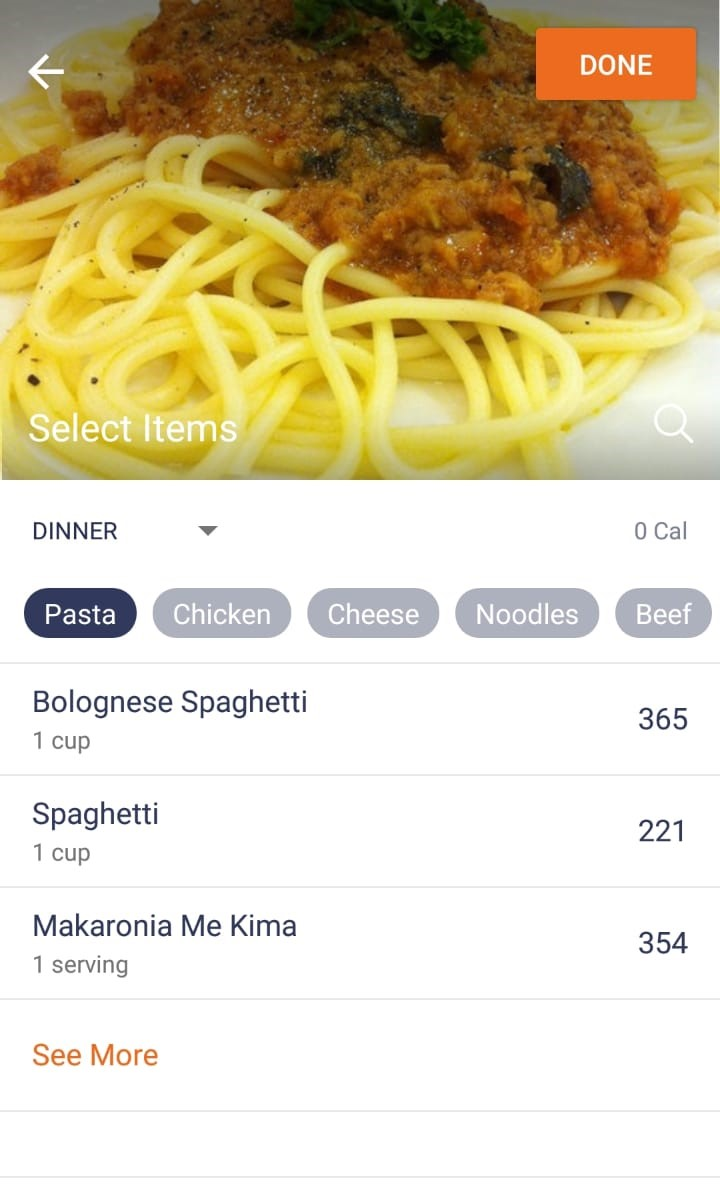
\includegraphics[width=\textwidth]{imgs/mama.jpeg}
  \label{fig:subApps1}
\end{subfigure}%
\hspace{.1\textwidth}
\begin{subfigure}{0.4\textwidth}
  \centering
    \caption{Aplicativo Lose It.}
  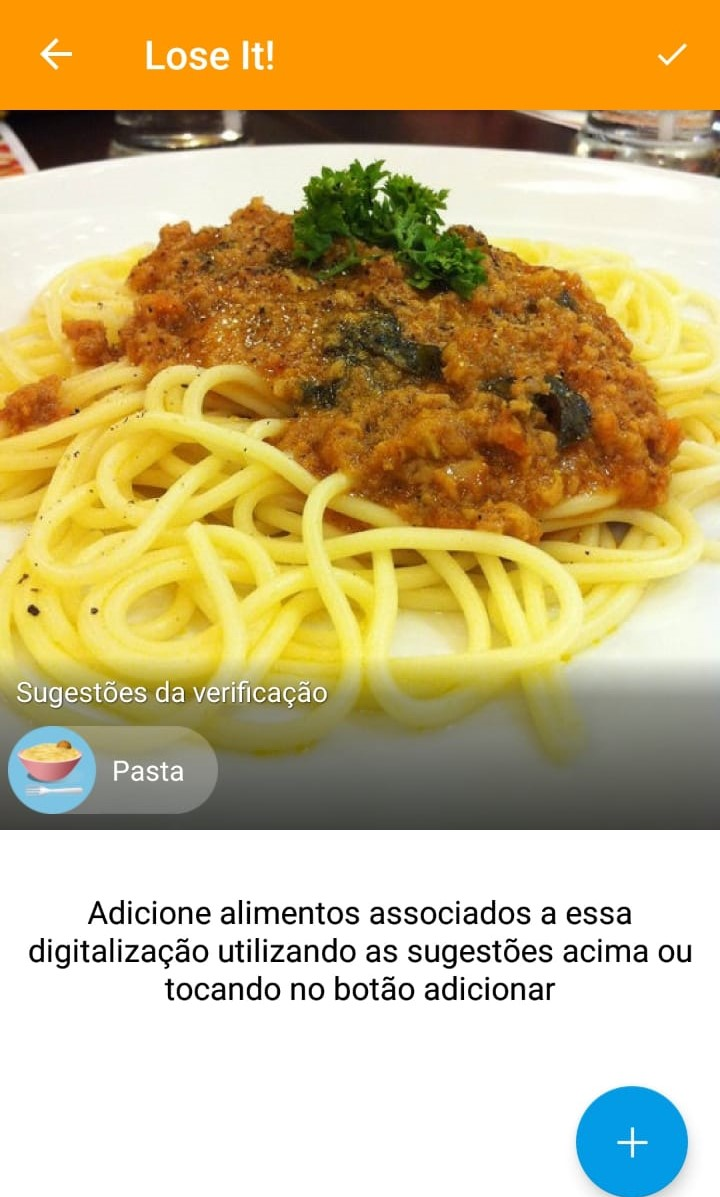
\includegraphics[width=\textwidth]{imgs/loseit.jpeg}
  \label{fig:subApps2}
\end{subfigure}

\label{fig:test}
\end{figure}


\subsection{Redes Neurais Artificias etc \label{subsec:nn}}

Redes Neurais Artificiais (RNA) são estruturas computacionais inspiradas no sistema nervoso de seres vivos. Essas estruturas são 
Neste capítulo, são apresentados alguns dos métodos detecção e reconhecimento de alimentos através de imagens. O objetivo aqui é descrever as vantagens e principais desvantagens desses métodos e seus respectivos resultados. 


\subsection{Detecção e Reconhecimento de Imagens}
A detecção e reconhecimento de imagens contendo alimentos são tópicos frequentemente pesquisados na área de visão computacional. Existem vários artigos publicados com diferentes abordagens para resolver esses dois problemas.  

\subsubsection{Detecção de Alimentos em Imagem}
A detecção de alimentos é diferente do reconhecimento alimentos, pois a primeira é uma classificação binária de imagens em imagens alimentares e não-alimentares, isto é, se contém comida ou não. Dada uma imagem, em que pode conter comida e fundo, a detecção de alimentos classifica a imagem como alimentar ou não-alimentar.

A Rede Neural Convolucional (CNN) oferece a mais recente técnica para muitos problemas gerais de classificação de imagem. Kagaya \cite{kagaya2014food} aplicou a CNN na classificação alimentar/não-alimentar e obteve resultados significativos com uma acurácia de 93,8\%. E, no trabalho \cite{kagaya2015highly}, a acurácia na detecção de alimentos foi aumentada para 99,1\%.

Esses resultados expressam que, em relação a trabalhos anteriores que utilizavam abordagens convencionais de aprendizado de máquina, a utilização de CNN aparenta mostrar uma melhor performance.

\subsubsection{Reconhecimento de Alimentos em Imagem}
A maioria dos trabalhos de pesquisa em reconhecimento de alimentos assumem que apenas um alimento está presente na imagem. Assim, o reconhecimento de alimentos pode ser resolvido como um problema de classificação multi-classes. 

A CNN também é amplamente utilizada no reconhecimento de alimentos e fornece melhor desempenho do que os métodos convencionais. 

Kagaya \cite{kagaya2014food} também treinou uma CNN para reconhecimento de alimentos e os resultados experimentais mostraram que a CNN superou todas as outras abordagens clássicas alcançando uma acurácia média de 73,7\% para 10 classes. Singla \cite{singla2016food} aplicou um modelo GoogLeNet pré-treinado baseado na arquitetura CNN nas tarefas de classificação de imagens alimentares/não-alimentares e para reconhecimento de categoria de alimentos. Os resultados experimentais mostram a precisão geral de 99,2\% na classificação alimentar/não-alimentar e 83,6\% na categorização de alimentos. 

A detecção e identificação de alimentos tem sido investigada na literatura em diferentes trabalhos, como os citados acima, inclusive \cite{aguilar2017food} e \cite{pouladzadeh2017cloud} em que foi evidenciado que os melhores resultados obtidos são baseados em Redes Neurais Convolucionais (CNN).






